\clearpage
\section{Trh půdy (definice, poptávka na trhu půdy, nabídka na trhu půdy, rovnováha na trhu,
pozemková renta).}

\subsection{Definice}
\begin{itemize}
    \item Půda je konečný faktor
    \item Půda není homogenní (kvalita a poloha se různí)
    \item \textbf{Pozemková renta} je důchod plynoucí z vlastnictví půdy v průběhu jejího využívání.
    \item Kvalita a poloha mohou vytvořit přírodní monopol (prodává se dráž než by odpovídalo nákladům).
\end{itemize}

\subsection{Poptávka na trhu půdy}
\begin{itemize}
    \item Jako u ostatních výrobních faktorů je to klesající křivka. Za malou rentu poptáváme hodně půdy,
    za vysokou rentu málo.
\end{itemize}

\subsubsection{Nabídka na trhu půdy}
\begin{itemize}
    \item Nabízený objem je konstantní.
\end{itemize}

\subsection{Rovnováha na trhu půdy}
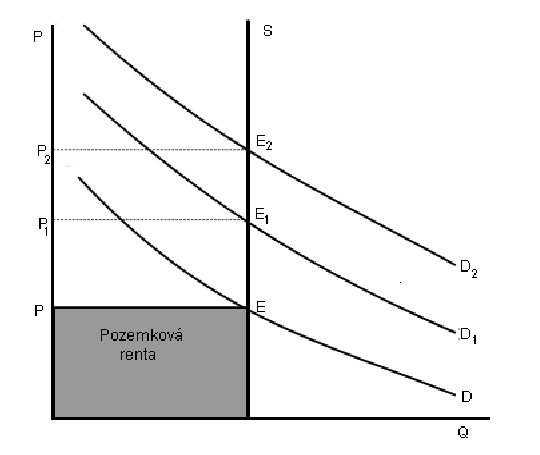
\includegraphics[]{images/19_rovnovaha.png}

\subsection{Pozemková renta}
\begin{itemize}
    \item Důchod plynoucí z vlastnictví půdy v průběhu jejího využívání
    \item Je to výnos z výrobního faktoru.
\end{itemize}